\documentclass[a4paper,12pt]{article}
 
% packages
\usepackage[T1]{fontenc}
\usepackage[latin1]{inputenc}
\usepackage{amsmath}
\usepackage{amsfonts}
\usepackage{amssymb}
\usepackage{graphicx}
\usepackage{listings}
\usepackage{url}
\usepackage[usenames]{xcolor}
\usepackage[top=3cm, bottom=3cm, left=3cm, right=3cm]{geometry}

% Path to the pictures
\graphicspath{ {images/} }

% Customized style to display c++ source code
\lstdefinestyle{customcpp}{
  backgroundcolor=\color{gray!15},
  belowcaptionskip=1\baselineskip,
  breaklines=true,
  frame=L,
  xleftmargin=\parindent,
  language=C++,
  showstringspaces=false,
  basicstyle=\footnotesize\ttfamily,
  keywordstyle=\bfseries\color{green!40!black},
  commentstyle=\itshape\color{purple!40!black},
  identifierstyle=\color{blue},
  stringstyle=\color{orange},
}
\lstset{style=customcpp}

% Title page definition

\makeatletter
\def\maketitle{%
  \null
  \thispagestyle{empty}%
  \begin{center}\leavevmode
    \normalfont
    {}
    \vskip 1.3cm
    {\Huge \@title\par}%
    \vskip 0.3cm
    {\Large Version: 0.8.0\par}%
    \vskip 0.3cm
    {\Large \@author\par}%
    \vskip 2cm
    {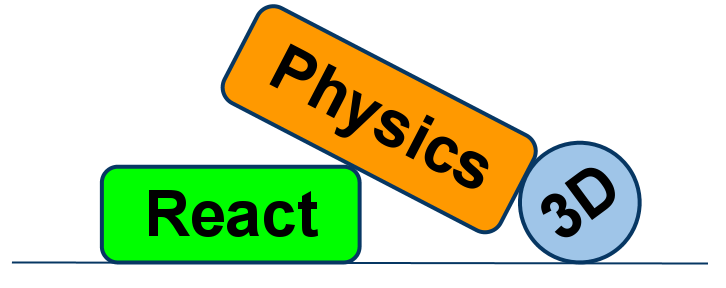
\includegraphics[height=5cm]{images/ReactPhysics3DLogo.png}}
    \vskip 2cm
    {\large{\url{http://www.reactphysics3d.com}}}
    \vskip 0.2cm
   {\large \@date}%
  \end{center}%
  \vfill
  \null
  \cleardoublepage
  }
\makeatother


\begin{document}
   \author{Daniel Chappuis}
   \title{ReactPhysics3D library \\ User Manual}
   \maketitle

   \tableofcontents

   \newpage
 

   \section{Introduction}

  ReactPhysics3D is an open source C++ physics engine library that can be used
  in 3D simulations and games. The library is released under the ZLib license.

   \section{Features}

   The ReactPhysics3D library has the following features :

   \begin{itemize}
    \item Rigid body dynamics 
    \item Discrete collision detection 
    \item Collision shapes (Sphere, Box, Cone, Cylinder, Capsule, Convex Mesh) 
    \item Broadphase collision detection (Sweep and Prune using AABBs) 
    \item Narrowphase collision detection (GJK/EPA) 
    \item Collision response and friction (Sequential Impulses Solver)
    \item Joints (Ball and Socket, Hinge, Slider, Fixed)
    \item Sleeping technique for inactive bodies
    \item Integrated Profiler 
    \item Multi-platform (Windows, Linux, Mac OS X)
    \item Documentation (User manual and Doxygen API)
    \item Examples
    \item Unit tests
   \end{itemize}

    \section{License}

    The ReactPhysics3D library is released under the open-source ZLib license. For more information, read the "LICENSE" file.

    \section{Building the library}
    \label{sec:building}

    You should use the CMake software to generate the makefiles or the 
    project files for your IDE. CMake can be downloaded at
    \url{http://www.cmake.org} or using you package-management program
    (apt, yum, \dots) on Linux. Then, you will be able to compile the library to create the static library
    file. In order to use ReactPhysics3D in your application, you can link your program with this static library.
    If you have never runned cmake, you should read the page \url{http://www.cmake.org/cmake/help/runningcmake.html} as
    it contains many useful information.

    \subsection{CMake using the command line (Linux and Mac OS X)}  

    Now, we will see how to build the ReactPhysics3D library using the CMake tool on the command line.
    First, create a folder into which you want to build the library. Then go into that folder and run
    the \texttt{ccmake} command : \\

    \texttt{ccmake \textless path\_to\_library\_source\textgreater} \\

    where \texttt{\textless path\_to\_library\_source\textgreater} must be replaced
    by the path the path to the \texttt{reactphysics3d-0.4.0/} folder. It is the folder that
    contains the \texttt{CMakeLists.txt} file. Running this command will launch the CMake command line interface.
    Hit the 'c' key to configure the project. There, you can also change some predefined variables (see section \ref{sec:cmakevariables} for more details)
    and then, hit the 'c' key again. Once you have set all the values as you like, you can hit the 'g' key to generate the makefiles in the build directory
    that you have created before and exit. \\

    Now that you have generated the makefiles with the CMake software, you can compile the code to build the static library in the
    \texttt{/lib} folder with the following command in your build directory : \\
    
    \texttt{make}

    \subsection{CMake using the graphical interface (Linux, Mac OS X and Windows)}

     Here, we will see how to build the ReactPhysics3D library using the CMake graphical interface. 
     First, run the \texttt{cmake-gui} program. The program will ask you for the
     source folder which is the \texttt{reactphysics3d-0.4.0/} folder of
     the library. You will also have to select a folder where you want to
     build the library and the examples. Select any empty folder that
     is on your system. Then, you can click on \texttt{Configure}. CMake will ask you to choose an IDE that is on
     your system. For instance, you can select Visual Studio, Qt Creator, XCode, ... Then you
     can change the compilation options. See section \ref{sec:cmakevariables} to see what are the possible options.
     Once this is done, you can click on \texttt{Configure} again and finally on \texttt{Generate}. \\ 
    
     Now, if you go into the folder you have chosen to build the
     library, you should be able to open the project file that corresponds to your IDE and compile
     the library.

     \subsection{CMake Variables}
     \label{sec:cmakevariables}

     You can find bellow the different CMake variables that you can set before generating the makefiles.

       \begin{description}
         \item[CMAKE\_BUILD\_TYPE] If this variable is set to DEBUG, the library will be compiled in debugging mode.
                                                    This mode should be used during development stage to know where things might crash.
                                                    In debugging mode, the library might run a bit slow due to all the debugging information
                                                    that are used. However, if this variable is set to RELEASE, no debugging information is stored
                                                    and therefore, it will run much faster. This mode must be used when you compile for the final
                                                    release of you application.
                                                   
         \item[COMPILE\_EXAMPLES] If this variable is ON, the examples of the reactphysics3d library will be compiled.
                                                    Note that you will need to have the Freeglut library installed on your system if you use
                                                    Windows or Linux and you will need to have the Glut library on Mac OS X if you want to
                                                    run those examples.

         \item[COMPILE\_TESTS] If this variable is ON, the unit tests of the reactphysics3d library will be compiled. You will then
                                             be able to launch the tests to make sure that they are running fine on your system.

          \item[PROFILING\_ENABLED] If this variable is ON, the integrated profiler will collect data will the application is running
                                                      and the profiling report will be display on the console at the end of the application (in the
                                                      destructor of the DynamicsWorld). This might be useful to see what part of the reactphysics3d
                                                      library takes time during its execution. This variable must be set to OFF when you compile
                                                      for the final release of your application.

          \item[DOUBLE\_PRECISION\_ENABLED] If this variable is ON, the reactphysics3d library will be compile with double floating point precision.
                                                                    Otherwise, the library will be compile with single precision.
       \end{description}
       

    \section{Using ReactPhysics3D in your application}

    In order to use the library in your own application, first build
    the static library of ReactPhysics3d as described above to get the
    static library file in the \texttt{lib/} folder. Then, in your code, you have to include
    the ReactPhysics3D header file with the line : \\

    \begin{lstlisting}
     // Include the ReactPhysics3D header file
     #include "reactphysics3d.h"
  \end{lstlisting}
   
    \vspace{0.6cm}

    Note that the \texttt{reactphysics3d.h} header file can be found in the
    \texttt{src/} folder of the library. Do not forget to add the
    \texttt{src/} folder in your include directories in order that the
    \texttt{reactphysics3d.h} file is accessible in your code. \\

    Do not forget to also link your application with the ReactPhysics3D
    static library.  \\
  
    Then, you should be able to compile your application using the
    ReactPhysics3D library. \\

    All the classes of the library are available in the \texttt{reactphysics3d} namespace or its shorter alias
    \texttt{rp3d}. Therefore, you need to include this namespace into your code with the following declaration : \\

    \begin{lstlisting}
     // Use the ReactPhysics3D namespace
     using namespace reactphysics3d;
  \end{lstlisting}

    \vspace{0.6cm}

    You should also take a look at the examples and the API documentation to get a better idea of how to use the
    ReactPhysics3D library.

    \section{The Physics World}

    The physics world will contain the bodies and joints that you create. You will then be able run the simulation across time by updating the world.
    The class \texttt{DynamicsWorld} represents the physics world in the ReactPhysics3D library.

    \subsection{Creating the Physics World}

    The first thing you have to do when you want to simulate dynamics of rigid bodies in time with the ReactPhysics3D library is to create an instance
    of the \texttt{DynamicsWorld}. You need to specify two parameters when constructing the world. The first one is the gravity acceleration  vector (in $m / s^2$) in the world and
    the second one is the simulation time step (in seconds). Note that gravity is activated by default when you create the world. The time step is the fixed amount of time that will be simulated
    each time a simulation step will be perform when updating the world. For real-time application, a time step of $\frac{1}{60}$ seconds (60 Hz) is usually used. Using a smaller time step
    makes the simulation more precise but also more expensive to compute. \\

    Here is how to create the world : \\

    \begin{lstlisting}
     // Gravity vector
     rp3d::Vector3 gravity(0.0, -9.81, 0.0);

     // Time step (in seconds)
     rp3d::decimal timeStep = 1.0 / 60.0;

     // Create the dynamics world
     rp3d::DynamicsWorld world(gravity, timeStep);
  \end{lstlisting}

    \subsection{Customizing the Physics World}

    \subsubsection{Solver parameters}

    ReactPhysics3D uses an iterative solver to solve contacts and joints. For contacts, there is a unique velocity solver and for joints there are a velocity and a
    position solver. By default, the number of iterations of the velocity solver is 10 and the number of iterations for the position solver is 5. It is possible to
    change the number of iterations for both solvers.

    To do this, you need to use the following two methods : \\

    \begin{lstlisting}
     // Change the number of iterations of the velocity solver
     world.setNbIterationsVelocitySolver(15);

     // Change the number of iterations of the position solver
     world.setNbIterationsPositionSolver(8);
  \end{lstlisting}

    \vspace{0.6cm}

    Increasing the number of iterations of the solvers will make the simulation more precise but also more expensive to compute. Therefore, you need to change
    those values only if needed.

    \subsubsection{Sleeping}

    The purpose of the sleeping technique is to deactivate resting bodies so that they are not simulated anymore. This is used to save computation because simulating many bodies is costly.
    A body (or group of bodies) is awaken as soon as another body collides with it or a joint in which it is involed is enabled. The sleeping technique is enabled by default. You can disable it
    using the following method : \\

    \begin{lstlisting}
     // Disable the sleeping technique
     world.enableSleeping(false);
  \end{lstlisting}

    \vspace{0.6cm}

    Note that it is not recommended to disable the sleeping technique because the simulating will become slower. It is also possible to deactivate the sleeping technique on a
    per body basis.

    // TODO : setSleepAngularVelocity and setSleepLinearVelocity, setTimeBeforeSleep()
    
    \subsection{Updating the Physics World}

    The first thing you have to do to simulate the dynamics of your world is to start the simulation using the following method : \\

    \begin{lstlisting}
     // Start the simulation
     world.start();
  \end{lstlisting}

    \vspace{0.6cm}

    Then, each time you have to compute the next frame to render in your application, you need to update the state of the world. To do that, you simply need to call this method : \\

    \begin{lstlisting}
     // Update the world by taking a simulation step
     world.update();
  \end{lstlisting}

    \vspace{0.6cm}

    When the \texttt{DynamicsWorld::update()} method is called, collision detection is performed and the position and orientation of the bodies are updated accordingly.
    After updating the world, you will be able to get the updated position and orientation of the bodies to render them in the next frame. Make sure that you call
    the \texttt{DynamicsWorld::start()} method before calling the \texttt{DynamicsWorld::update()} method. \\

    You can also use the \texttt{DynamicsWorld::stop()} method to stop the simulation. You will then be able to start it again and to continue updating it. \\

    Note that you can get the elapsed time (in seconds) from the beginning of the physics simulation using the \texttt{DynamicsWorld::getPhysicsTime()} method. This can be useful to
    create some animations.

    \subsection{Destroying the Physics World}

    Do not forget to destroy the \texttt{DynamicsWorld} instance at the end of your program in order to release the allocated memory. If the object has been created statically, it will
    automatically be destroy at the end of the scope in which it has been created. If the object has been created dynamically (using the \texttt{new} operator), you need to destroy
    it with the \texttt{delete} operator.

    \section{Rigid Bodies}

    Once the physics world has been created, you can create rigid bodies into the world. A rigid body will represent the objects you want to simulate in the physics world.
    A rigid body has a mass, a collision shape, a position and an orientation. The physics world will compute collision between the bodies and will update their position and
    orientation accordingly at each time step. You can also create joints between the bodies in the world. In ReactPhysics3D, the class \texttt{RigidBody} is used to describe a rigid body.

    \subsection{Creating a Rigid Body}

    In order to create a rigid body, you need to specify a transform, its mass, its inertia tensor and a collision shape. The transform describes the initial
    position and orientation of the body in the world. To do that, you need to create an instance of the \texttt{Transform} with a vector describing the
    initial position and a quaternion for the initial orientation of the body. \\

    In order that your rigid body can collide with other bodies in the world, you need to specify a collision shape. Take a look at section \ref{sec:collisionshapes} to learn about the
    different collision shapes and how to create them. \\

    To create a rigid body, you also need to give the mass of the body (in kilograms) and inertia tensor. The inertia tensor is a $3 \times 3$ matrix decribing how the mass is
    distributed inside the rigid body which will be used to calculate the rotation of the body. The inertia tensor can be calculate from the collision shape that you have created for the
    body. You can find more information about this in section \ref{sec:inertiacollisionshape}. \\

    You need to call the \texttt{DynamicsWorld::createRigidBody()} method to create a rigid body in the world previously created. This method will return a pointer to the instance
    of the \texttt{RigidBody} class that has been created internally. You will then be able to use that pointer to get or set values to the body. \\

    You can see in the following code how to create a rigid body with a box collision shape : \\

    \begin{lstlisting}
     // Create the collision shape of the rigid body
     const rp3d::BoxShape collisionShape(rp3d::Vector3(1.0, 1.0, 1.0));

     // Compute the inertia tensor of the body
     rp3d::Matrix3x3 inertiaTensor;
     collisionShape.computeLocalInertiaTensor(inertiaTensor, mass);

     // Initial position and orientation of the rigid body
     rp3d::Vector3 initPosition(0.0, 3.0, 0.0);
     rp3d::Quaternion initOrientation = rp3d::Quaternion::identity();
     rp3d::Transform transform(initPosition, initOrientation);

     // Create a rigid body in the world
     rp3d::RigidBody* body;
     body = dynamicsWorld->createRigidBody(transform, mass, inertiaTensor, collisionShape);
  \end{lstlisting}

    \subsection{Customizing a Rigid Body}

    TODO : Damping

    \subsection{Updating a Rigid Body}

    When you call the \texttt{DynamicsWorld::update()} method, the collision between the bodies are computed and the joints are evaluated. Then, the bodies position and orientation
    are updated accordingly. After calling this method, you can get the updated position and orientation of each body to render it. To do that, you simply need to use the
    \texttt{RigidBody::getInterpolatedTransform()} method to get the interpolated transform. This transform represents the current local-to-world-space transformation. \\

    Here is how to get the interpolated transform of a rigid body : \\

    \begin{lstlisting}
     // Here, body is a RigidBody* pointer previously created

     // Get the interpolated transform of the rigid body
     rp3d::Transform transform = body->getInterpolatedTransform();
  \end{lstlisting}

    \vspace{0.6cm}

    If you need the array with the corresponding $4 \times 4$ OpenGL transformation matrix, you can use the \texttt{Transform::getOpenGLMatrix()} method as in the following code : \\

    \begin{lstlisting}
   // Get the OpenGL matrix array of the transform
   float matrix[16];
   transform.getOpenGLMatrix(matrix);
  \end{lstlisting}

    \subsection{Destroying a Rigid Body}

    \begin{sloppypar}
    It is really simple to destroy a rigid body. You simply need to use the \texttt{DynamicsWorld::destroyRigidBody()} method. You need to use the pointer to the body you
    want to destroy as argument. Note that after calling that method, the pointer will not be valid anymore and therefore, you should not use it. Note that you must
    destroy all the rigid bodies at the end of the simulation before you destroy the world. When you destroy a rigid body that was part of a joint, that joint will be automatically
    destroyed as well. \\
    \end{sloppypar}

    Here is how to destroy a rigid body : \\

    \begin{lstlisting}
     // Here, world is an instance of the DynamicsWorld class
     // and body is a RigidBody* pointer

     // Destroy the rigid body
    world.destroyRigidBody(body);
  \end{lstlisting}

    \section{Collision Shapes}
    \label{sec:collisionshapes}

    When you create a rigid body, you need to specify a collision shape. This shape will be used to test collision between the body and its environment.
    This section describes all the collision shapes available in the ReactPhysics3D library and how to use them. \\

    Every collision shapes use a \emph{collision margin} which is a small distance around the shape that is used internally in the collision detection.
    Some collision shapes have their collision margin integrated into the shape that you define and therefore you do not have to worry about it.
    However, for some collision shapes, the collision margin is added around the shape that you define and therefore, you might have to compensate
    for this small margin with the way you render the object. \\

    Once you have created a collision shape object, you need to used it when you create a rigid body in the physics world using the
    \texttt{DynamicsWorld::createRigidBody()} method. Note that during the rigid body creating, the collision shape object that you gave as a parameter
    will be copied internally. Therefore, you can destroy the collision shape object right after the rigid body creation.

    \subsection{Box Shape}

    \begin{figure}[h]
        \centering
        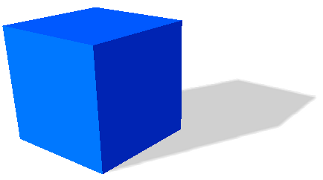
\includegraphics{boxshape.png}
        \label{fig:boxshape}
    \end{figure}

    The class \texttt{BoxShape} class describes a box collision shape centered at the origin of the body local space. The box is aligned with the local x, y and z axis.
    In order to create a box shape, you only need to specify the three half extents dimensions of the box in the three X, Y and Z directions. \\

    For instance, if you want to create a box shape with dimensions of 4 meters, 6 meters and 10 meters along the X, Y and Z axis respectively, you need to use the following code : \\

    \begin{lstlisting}
     // Half extents of the box in the x, y and z directions
     const rp3d::Vector3 halfExtents(2.0, 3.0, 5.0);

     // Create the box shape
     const rp3d::BoxShape boxShape(halfExtents);
  \end{lstlisting}

    \vspace{0.6cm}

    The \texttt{BoxShape} has a collision margin that is added to the box dimension you define. Therefore, the actual box shape will be a little bit larger that the one you define.
    It is recommended that you use the default margin. In case, you really need to change the collision margin of your box shape (if the dimension of your box is small compared
    to the default collision margin for instance), you can pass the length of the new collision margin (in meters) as a second parameter of the BoxShape constructor. \\

    For instance, if you want to use a collision margin of 1 centimeter for your box shape, you can do it like this : \\

   \begin{lstlisting}
     // Create the box shape with a custom collision margin
     const rp3d::BoxShape boxShape(halfExtents, 0.01);
  \end{lstlisting}

    \subsection{Sphere Shape}

    \begin{figure}[h]
        \centering
        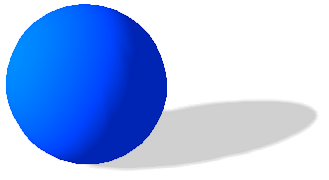
\includegraphics{sphereshape.png}
        \label{fig:sphereshape}
    \end{figure}

    The \texttt{SphereShape} class describes a sphere collision shape centered at the origin of the body local space. You only need to specify the radius of sphere to create it. \\

    For instance, if you want to create a sphere shape with a radius of 2 meters, you need to use the following code : \\

    \begin{lstlisting}
     // Create the sphere shape with a radius of 2m
     const rp3d::SphereShape sphereShape(2.0);
  \end{lstlisting}

    \vspace{0.6cm}

    The collision margin of the \texttt{SphereShape} is integrated into the sphere you define. Therefore, you do not need to worry about it and you cannot change it.

    \subsection{Cone Shape}

    \begin{figure}[h]
        \centering
        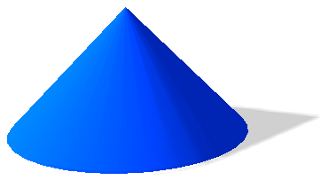
\includegraphics{coneshape.png}
        \label{fig:coneshape}
    \end{figure}

    The \texttt{ConeShape} class describes a cone collision shape centered at the origin of the body local-space. The cone is aligned along the Y axis.
    In order to create a cone shape, you need to give the radius of the base of the cone and the height of the cone (along the Y axis). \\

    For instance, if you want to create a cone shape with a radius of 1 meter and the height of 3 meters, you need to use the following code : \\

    \begin{lstlisting}
     // Create the cone shape
     const rp3d::ConeShape coneShape(1.0, 3.0);
  \end{lstlisting}

    \vspace{0.6cm}

    The \texttt{ConeShape} has a collision margin that is added to the cone dimension that you define. Therefore, the actual cone shape will be a little bit larger that the one you define.
    It is recommended that you use the default margin. In case, you really need to change the collision margin of your cone shape (if the dimension of your cone is small compared
    to the default collision margin for instance), you can pass the length of the new collision margin (in meters) as a third parameter of the \texttt{ConeShape} constructor. \\

    For instance, if you want to use a collision margin of 1 centimeter for your cone shape, you can do it like this : \\

   \begin{lstlisting}
     // Create the cone shape with a custom collision margin
     const rp3d::ConeShape coneShape(1.0, 3.0, 0.01);
  \end{lstlisting}

    \subsection{Cylinder Shape}

    \begin{figure}[h]
        \centering
        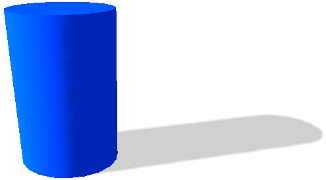
\includegraphics{cylindershape.png}
        \label{fig:cylindershape}
    \end{figure}

    The \texttt{CylinderShape} class describes a cylinder collision shape centered at the origin of the body local-space. The cylinder is aligned along the Y axis.
    In order to create a cylinder shape, you need to specify the radius of the base and the height of the cylinder (along the Y axis). \\

    For instance, if you want to create a cylinder shape with a radius of 1 meter and the height of 3 meters, you need to use the following code : \\

    \begin{lstlisting}
     // Create the cylinder shape
     const rp3d::Cylinder cylinderShape(1.0, 3.0);
  \end{lstlisting}

    \vspace{0.6cm}

    The \texttt{CylinderShape} has a collision margin that is added to the cylinder dimension that you define. Therefore, the actual cylinder shape will be a little bit larger that the one you define.
    It is recommended that you use the default margin. In case, you really need to change the collision margin of your cylinder shape (if the dimension of your cylinder is small compared
    to the default collision margin for instance), you can pass the length of the new collision margin (in meters) as a third parameter of the \texttt{CylinderShape} constructor. \\

    For instance, if you want to use a collision margin of 1 centimeter for your cylinder shape, you can do it like this : \\

   \begin{lstlisting}
     // Create the cylinder shape with a custom collision margin
     const rp3d::CylinderShape cylinderShape(1.0, 3.0, 0.01);
  \end{lstlisting}

    \subsection{Capsule Shape}

    \begin{figure}[h]
        \centering
        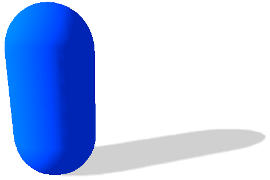
\includegraphics{capsuleshape.png}
        \label{fig:capsuleshape}
    \end{figure}

    The \texttt{CapsuleShape} class describes a capsule collision shape around the Y axis and centered at the origin of the body local space. It is the convex hull of two
    spheres. It can also be seen as an elongated sphere. In order to create it, you only need to specify the radius of the two spheres and the height of the
    capsule (distance between the centers of the two spheres).  \\

    For instance, if you want to create a capsule shape with a radius of 1 meter and the height of 2 meters, you need to use the following code : \\

    \begin{lstlisting}
     // Create the capsule shape
     const rp3d::CapsuleShape capsuleShape(1.0, 2.0);
  \end{lstlisting}

    \vspace{0.6cm}

    As for the \texttt{SphereShape}, the collision margin of the \texttt{CapsuleShape} is integrated into the capsule you define.
    Therefore, you do not need to worry about it and you cannot change it.

    \subsection{Convex Mesh Shape}

    \begin{figure}[h]
        \centering
        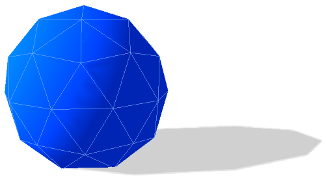
\includegraphics{convexshape.png}
        \label{fig:convexshape}
    \end{figure}

    The class \texttt{ConvexMeshShape} can be used to describe the shape of a convex mesh. In order to create a convex mesh shape, you need to supply the array with the coordinates of
    the vertices of the mesh. The array is supposed to start with the three X, Y and Z coordinates of the first vertex, then the X, Y and Z coordinates of the second vertex and so on.
    The first parameter of the \texttt{ConvexMeshShape} constructor is a pointer to the array of vertices coordinates, the second parameter is the number of vertices in the array and
    the third parameter is the size (in bytes) of the data needed for a single vertex in the array (data used by all the three coordinates of a single vertex).

    \begin{lstlisting}
    // Construct a convex mesh shape
    rp3d::ConvexMeshShape shape(verticesArray, nbVertices, 3 * sizeof(float));
  \end{lstlisting}

    \vspace{0.6cm}

    You need to make sure that the mesh you provide is indeed convex and also that the its origin of its local-space is inside the mesh. \\

    The collision detection test with a convex mesh shape runs in $O(n)$ where $n$ is the number of vertices in the mesh. Collision detection can become expensive if there are
    too many vertices in the mesh. It is possible to speed up the collision detection by providing information about the edges of the convex mesh. If you provide edges information
    about the convex mesh, the collision detection will run in almost constant time at the cost of a little extra memory to store the edges information. In order to provide the edges
    information, you need to call the \texttt{ConvexMeshShape::addEdge()} method for each edge of the mesh. The first parameter is the index of the first vertex of the edge and the
    second parameter is the index of the second vertex. Do not worry about calling this method multiple times for the same edge, the edge information will be added only
    once. \\

    For instance, the following code adds the edges information into a convex mesh shape : \\

    \begin{lstlisting}
    // Add the edges information of the mesh into the shape
    for (unsigned int i=0; i<mesh.getNbFaces(); i++) {

        // Get the three vertex IDs of the vertices of the face
        unsigned int v1 = getVertexIndexInFace(i, 0);
        unsigned int v2 = getVertexIndexInFace(i, 1);
        unsigned int v3 = getVertexIndexInFace(i, 2);

        // Add the three edges into the collision shape
        convexShape.addEdge(v1, v2);
        convexShape.addEdge(v1, v3);
        convexShape.addEdge(v2, v3);
    }
  \end{lstlisting}

    \vspace{0.6cm}

    Do not forget to enable the fast collision detection by asking the collision shape to use the edges information you have just provided. To do this, you need to
    call the \texttt{ConvexMeshShape::setIsEdgesInformation()} method as in the following example : \\

     \begin{lstlisting}
    // Enable the fast collision detection
    // using the edges information
    collisionShape.setIsEdgesInformationUsed(true);
  \end{lstlisting}

    \subsection{Inertia Tensor of a Collision Shape}
    \label{sec:inertiacollisionshape}

    When you create a rigid body, you need to specify its inertia tensor. The inertia tensor is a $3 \times 3$ matrix decribing how the mass is distributed inside the rigid body which
    will be used to calculate the rotation of the body. The inertia tensor depends on the mass and the shape of the body. \\

    You can use the collision shape of a rigid body to compute its inertia tensor. To do that, you need to use the \texttt{CollisionShape::computeLocalInertiaTensor()} method of your collision
    shape. This method takes two parameters. The first one if the inertia tensor matrix that need to be computed and the second one is the mass of the rigid body (in kilograms). For instance,
    if you want to compute the inertia tensor matrix of a capsule shape with a mass of 3 kilograms, here is what the code looks like : \\

    \begin{lstlisting}
     // Compute the inertia tensor of a rigid body
    rp3d::Matrix3x3 inertiaTensor;
    capsuleShape.computeLocalInertiaTensor(inertiaTensor, 3.0);
  \end{lstlisting}

    \section{Joints}

    Joints are used to constraint the motion of the rigid bodies between each other. A single joint represents a constraint between two rigid bodies.
    When the motion of the first body of the joint is known, the relative motion of the second body has at most six degrees of freedom (three for the
    translation and three for the rotation). The different joints can reduce the number of degrees of freedom between two rigid bodies. \\

    Some joints have limits to control the range of motion and some joints have motors to automatically move the the bodies of the joint at a given speed. \\
    
    \subsection{Ball and Socket Joint}

    The \texttt{BallAndSocketJoint} class describes a ball and socket joint between two bodies. In a ball and socket joint, the two bodies cannot translate with respect to each other.
    However, they can rotate freely around a common anchor point. This joint has three degrees of freedom. This joint can be used to simulate a chain of bodies for instance. \\

    In order to create a ball and socket joint, you first need to create an object of the \texttt{BallAndSocketJointInfo} class with the necessary information. You need to provide the pointers to the
    two rigid bodies and also the coordinates of the anchor point (in world-space). At the joint creation, the world-space anchor point will be converted into the local-space of the two rigid
    bodies and then, the joint will make sure that the two local-space anchor points match in world-space. Therefore, the two bodies need to be in a correct position at the joint creation. \\

    Here is the code to create the \texttt{BallAndSocketJointInfo} object : \\

    \begin{lstlisting}
     // Anchor point in world-space
     const rp3d::Vector3 anchorPoint(2.0, 4.0, 0.0);

     // Create the joint info object
     rp3d::BallAndSocketJointInfo jointInfo(body1, body2, anchorPoint);
  \end{lstlisting}

    \vspace{0.6cm}

    Now, it is time to create the actual joint in the dynamics world using the \texttt{DynamicsWorld::createJoint()} method.
    Note that this method will also return a pointer to the \texttt{BallAndSocketJoint} object that has been created internally. You will then
    be able to use that pointer to change properties of the joint and also to destroy it at the end. \\

    Here is how to create the joint in the world : \\

    \begin{lstlisting}
     // Create the joint in the dynamics world
     rp3d::BallAndSocketJoint* joint;
     joint = dynamic_cast<rp3d::BallAndSocketJoint*>(world.createJoint(jointInfo));
  \end{lstlisting}

    \vspace{0.6cm}

    \subsection{Hinge Joint}

    The class \texttt{HingeJoint} describes a hinge joint (or revolute joint) between two rigid bodies. The hinge joint only allows rotation around an anchor point and
    around a single axis (the hinge axis). This joint can be used to simulate doors or pendulums for instance. \\

    In order to create a hinge joint, you first need to create a \texttt{HingeJointInfo} object with the necessary information. You need to provide the pointers to the
    two rigid bodies, the coordinates of the anchor point (in world-space) and also the hinge rotation axis (in world-space). The two bodies need to be in a correct position
    when the joint is created. \\

    Here is the code to create the \texttt{HingeJointInfo} object : \\

    \begin{lstlisting}
     // Anchor point in world-space
     const rp3d::Vector3 anchorPoint(2.0, 4.0, 0.0);

     // Hinge rotation axis in world-space
     const rp3d::Vector3 axis(0.0, 0.0, 1.0);

     // Create the joint info object
     rp3d::HingeJointInfo jointInfo(body1, body2, anchorPoint, axis);
  \end{lstlisting}

    \vspace{0.6cm}

    Now, it is time to create the actual joint in the dynamics world using the \texttt{DynamicsWorld::createJoint()} method.
    Note that this method will also return a pointer to the \texttt{HingeJoint} object that has been created internally. You will then
    be able to use that pointer to change properties of the joint and also to destroy it at the end. \\

    Here is how to create the joint in the world : \\

    \begin{lstlisting}
     // Create the hinge joint in the dynamics world
     rp3d::HingeJoint* joint;
     joint = dynamic_cast<rp3d::HingeJoint*>(world.createJoint(jointInfo));
  \end{lstlisting}

     \subsubsection{Limits}

     With the hinge joint, you can constraint the motion range using limits. The limits of the hinge joint are the minimum and maximum angle of rotation allowed with respect to the initial
     angle between the bodies when the joint is created. The limits are disabled by default. If you want to use the limits, you first need to enable them by setting the
     \texttt{isLimitEnabled} variable of the \texttt{HingeJointInfo} object to \emph{true} before you create the joint. You also have to specify the minimum and maximum limit
     angles (in radians) using the \texttt{minAngleLimit} and \texttt{maxAngleLimit} variables of the joint info object. Note that the minimum limit angle must be in the
     range $[ -2 \pi; 0 ]$ and the maximum limit angle must be in the range $[ 0; 2 \pi ]$. \\

     For instance, here is the way to use the limits for a hinge joint when the joint is created : \\

     \begin{lstlisting}
     // Create the joint info object
     rp3d::HingeJointInfo jointInfo(body1, body2, anchorPoint, axis);

     // Enable the limits of the joint
     jointInfo.isLimitEnabled = true;

     // Minimum limit angle
     jointInfo.minAngleLimit = -PI / 2.0;

     // Maximum limit angle
     jointInfo.maxAngleLimit = PI / 2.0;

      // Create the hinge joint in the dynamics world
     rp3d::HingeJoint* joint;
     joint = dynamic_cast<rp3d::HingeJoint*>(world.createJoint(jointInfo));
  \end{lstlisting}

     \vspace{0.6cm}

     \begin{sloppypar}
        It is also possible to use the \texttt{HingeJoint::enableLimit()}, \texttt{HingeJoint::setMinAngleLimit()} and \texttt{HingeJoint::setMaxAngleLimit()} methods to specify
        the limits of the joint after its creation. See the API documentation for more information.
     \end{sloppypar}

     \subsubsection{Motor}

     A motor is also available for the hinge joint. It can be used rotate the bodies around the hinge axis at a given angular speed and such that the torque applied to
     rotate the bodies does not exceed a maximum allowed torque. The motor is disabled by default. If you want to use it, you first have to activate it using the
     \texttt{isMotorEnabled} boolean variable of the \texttt{HingeJointInfo} object before you create the joint. Then, you need to specify the angular motor speed (in radians/seconds)
     using the \texttt{motorSpeed} variable and also the maximum allowed torque (in Newton $\cdot$ meters) with the \texttt{maxMotorTorque} variable. \\

     For instance, here is how to enable the motor of the hinge joint when the joint is created : \\

     \begin{lstlisting}
     // Create the joint info object
     rp3d::HingeJointInfo jointInfo(body1, body2, anchorPoint, axis);

     // Enable the motor of the joint
     jointInfo.isMotorEnabled = true;

     // Motor angular speed
     jointInfo.motorSpeed = PI / 4.0;

     // Maximum allowed torque
     jointInfo.maxMotorTorque = 10.0;

      // Create the hinge joint in the dynamics world
     rp3d::HingeJoint* joint;
     joint = dynamic_cast<rp3d::HingeJoint*>(world.createJoint(jointInfo));
  \end{lstlisting}

     \vspace{0.6cm}

     \begin{sloppypar}
        It is also possible to use the \texttt{HingeJoint::enableMotor()}, \texttt{HingeJoint::setMotorSpeed()} and \texttt{HingeJoint::setMaxMotorTorque()} methods to
        enable the motor of the joint after its creation. See the API documentation for more information.
     \end{sloppypar}

    \subsection{Slider Joint}

    The class \texttt{SliderJoint} describes a slider joint (or prismatic joint) that only allows relative translation along a single direction. It has a single degree of freedom and allows no
    relative rotation. In order to create a slider joint, you first need to specify the anchor point (in world-space) and the slider axis direction (in world-space). The constructor of the
    \texttt{SliderJointInfo} object needs two pointer to the bodies of the joint, the anchor point and the axis direction. Note that the two bodies have to be in a correct initial position when
    the joint is created. \\

    You can see in the following code how to specify the information to create a slider joint : \\

    \begin{lstlisting}
     // Anchor point in world-space
     const rp3d::Vector3 anchorPoint = rp3d::decimal(0.5) * (body2Position + body1Position);

     // Slider axis in world-space
    const rp3d::Vector3 axis = (body2Position - body1Position);

    // Create the joint info object
    rp3d::SliderJointInfo jointInfo(body1, body2, anchorPoint, axis);
  \end{lstlisting}

    \vspace{0.6cm}

    Now, it is possible to create the actual joint in the dynamics world using the \texttt{DynamicsWorld::createJoint()} method.
    Note that this method will also return a pointer to the \texttt{SliderJoint} object that has been created internally. You will then
    be able to use that pointer to change properties of the joint and also to destroy it at the end. \\

    Here is how to create the joint in the world : \\

    \begin{lstlisting}
     // Create the slider joint in the dynamics world
     rp3d::SliderJoint* joint;
     joint = dynamic_cast<rp3d::SliderJoint*>(world.createJoint(jointInfo));
  \end{lstlisting}

    \subsubsection{Limits}

    It is also possible to control the range of the slider joint motion using limits. The limits are disabled by default. In order to use the limits when the joint is created, you first
    need to activate them using the \texttt{isLimitEnabled} variable of the \texttt{SliderJointInfo} class. Then, you need to specify the minimum and maximum translation limits
    (in meters) using the \texttt{minTranslationLimit} and \texttt{maxTranslation\-Limit} variables. Note that the initial position of the two bodies when the joint is created
    corresponds to a translation of zero. Therefore, the minimum limit must be smaller or equal to zero and the maximum limit must be larger or equal to zero. \\

    You can see in the following example how to set the limits when the slider joint is created : \\

    \begin{lstlisting}
     // Create the joint info object
     rp3d::SliderJointInfo jointInfo(body1, body2, anchorPoint, axis);

     // Enable the limits of the joint
     jointInfo.isLimitEnabled = true;

     // Minimum translation limit
     jointInfo.minTranslationLimit = -1.7;

     // Maximum translation limit
     jointInfo.maxTranslationLimit = 1.7;

      // Create the hinge joint in the dynamics world
     rp3d::SliderJoint* joint;
     joint = dynamic_cast<rp3d::SliderJoint*>(world.createJoint(jointInfo));
  \end{lstlisting}

    \vspace{0.6cm}
 
   \begin{sloppypar}
    You can also use the \texttt{SliderJoint::enableLimit()}, \texttt{SliderJoint::\-setMinTranslationLimit()} and \texttt{SliderJoint::setMaxTranslationLimit()} methods to enable the
    limits of the joint after its creation. See the API documentation for more information.
    \end{sloppypar}

    \subsubsection{Motor}

     The slider joint also has a motor. You can use it to translate the bodies along the slider axis at a given linear speed and such that the force applied to
     move the bodies does not exceed a maximum allowed force. The motor is disabled by default. If you want to use it when the joint is created, you first have to activate it using the
     \texttt{isMotorEnabled} boolean variable of the \texttt{SliderJointInfo} object before you create the joint. Then, you need to specify the linear motor speed (in meters/seconds)
     using the \texttt{motorSpeed} variable and also the maximum allowed force (in Newtons) with the \texttt{maxMotorForce} variable. \\

     For instance, here is how to enable the motor of the slider joint when the joint is created : \\

     \begin{lstlisting}
     // Create the joint info object
     rp3d::SliderJointInfo jointInfo(body1, body2, anchorPoint, axis);

     // Enable the motor of the joint
     jointInfo.isMotorEnabled = true;

     // Motor linear speed
     jointInfo.motorSpeed = 2.0;

     // Maximum allowed force
     jointInfo.maxMotorForce = 10.0;

      // Create the slider joint in the dynamics world
     rp3d::SliderJoint* joint;
     joint = dynamic_cast<rp3d::SliderJoint*>(world.createJoint(jointInfo));
  \end{lstlisting}

     \vspace{0.6cm}

     \begin{sloppypar}
        It is also possible to use the \texttt{SliderJoint::enableMotor()}, \texttt{SliderJoint::setMotorSpeed()} and \texttt{SliderJoint::setMaxMotorForce()} methods to enable the
        motor of the joint after its creation. See the API documentation for more information.
     \end{sloppypar}

    \subsection{Fixed Joint}

    The class \texttt{FixedJoint} describes a fixed joint between two bodies. In a fixed joint, there is no degree of freedom, the bodies are not allowed to translate
    or rotate with respect to each other. In order to create a fixed joint, you simply need to specify an anchor point (in world-space) to create the \texttt{FixedJointInfo}
    object. \\

    For instance, here is how to create the joint info object for a fixed joint : \\

    \begin{lstlisting}
     // Anchor point in world-space
     rp3d::Vector3 anchorPoint(2.0, 3.0, 4.0);

     // Create the joint info object
     rp3d::FixedJointInfo jointInfo1(body1, body2, anchorPoint);
  \end{lstlisting}

    \vspace{0.6cm}

    Now, it is possible to create the actual joint in the dynamics world using the \texttt{DynamicsWorld::createJoint()} method.
    Note that this method will also return a pointer to the \texttt{FixedJoint} object that has been created internally. You will then
    be able to use that pointer to change properties of the joint and also to destroy it at the end. \\

    Here is how to create the joint in the world : \\

    \begin{lstlisting}
     // Create the fixed joint in the dynamics world
     rp3d::FixedJoint* joint;
     joint = dynamic_cast<rp3d::FixedJoint*>(world.createJoint(jointInfo));
  \end{lstlisting}

    \subsection{Collision between the bodies of a Joint}

    By default the two bodies involved in a joint are able to collide with each other. However, it is possible to disable the collision between the two bodies that are part
    of the joint. To do it, you simply need to set the variable \texttt{isCollisionEnabled} of the joint info object to \emph{false} when you create the joint. \\

    For instance, when you create a \texttt{HingeJointInfo} object in order to construct a hinge joint, you can disable collision between the two bodies of the joint as in the
    following example : \\

    \begin{lstlisting}
     // Create the joint info object
     rp3d::HingeJointInfo jointInfo(body1, body2, anchorPoint, axis);

     // Disable the collision between the bodies
     jointInfo.isCollisionEnabled = false;

     // Create the joint in the dynamics world
     rp3d::HingeJoint* joint;
     joint = dynamic_cast<rp3d::HingeJoint*>(world.createJoint(jointInfo));
  \end{lstlisting}

    \subsection{Destroying a Joint}

    In order to destroy a joint, you simply need to call the \texttt{DynamicsWorld::destroyJoint()} method using the pointer to
    a previously created joint object as argument as shown in the following code : \\

    \begin{lstlisting}
     // rp3d::BallAndSocketJoint* joint is a previously
     // created joint

     // Destroy the joint
     world.destroyJoint(joint);
  \end{lstlisting}

    \vspace{0.6cm}

    It is important that you destroy all the joints that you have created at the end of the simulation. Also note that destroying a
    rigid body that is involved in a joint will automatically destroy that joint.

    \section{Examples}

    You can find some demos in the \texttt{examples/} folder of
    the reactphysics3d library. Follow the instructions described in section \ref{sec:building} to
    compile the examples. Note that the FREEGLUT library is required on Linux and Windows
    and the GLUT library is required on Mac OS X to run those examples. Studying the examples is a
    good way to understand how to use the reactphysics3d library.

    \subsection{Cubes}

    In this examples, you will see how to create a floor and some cubes using the Box Shape for collision detection. Because of gravity,
    the cubes will fall down on the floor. After falling down, the cubes will come to rest and start sleeping (become inactive). In this demo,
    the cubes are green when they are inactive and become red as they get inactive (sleeping).

    \subsection{Collision Shapes}

    In this example, you will see how to create a floor (using the Box Shape) and some other bodies using the different collision shapes available
    in the reactphysics3d library like Cylinders, Capsules, Spheres, Convex Meshes and Cones. Those bodies will fall down to the floor.

    \subsection{Joints}

    In this example, you will learn how to create different joints (Ball and Socket, Hinge, Slider, Fixed) into the dynamics world. You can also see how
    to set the motor or limits of the joints.

    \section{Receiving Feedback}

    \subsection{Contacts}

    \section{Profiler}

   \section{API Documentation}

   Some documentation about the API of the code has been generated
   using Doxygen. You will be able to find this documentation in the library archive in the folder \texttt{/documentation/API/html/}. You just
   need to open the \texttt{index.html} file with your favorite web browser.

    \section{Bugs}

    If you find some bugs, do not hesitate to report them on the issue tracker of the ReactPhysics3D website at : \\

    \url{http://code.google.com/p/reactphysics3d/issues/list} \\

    Thanks a lot for reporting the bugs that you find. It will help us to correct and improve the library.
   
\end{document}
